\documentclass[sigconf,natbib=false,10pt]{acmart}
\settopmatter{printacmref=false}
\setcopyright{none}
\renewcommand\footnotetextcopyrightpermission[1]{}

\acmConference[SOSP '25]{Symposium on Operating Systems Principles}{October
2025}{Seoul, Republic of Korea}


% to be able to draw some self-contained figs
\usepackage{tikz}
\usepackage{amsmath}
\usepackage{hyperref}
\usepackage[normalem]{ulem}
\usepackage{listings}
\usepackage{xspace}
\usepackage{booktabs}
\usepackage{multirow}
% \usepackage{wasysym}
\usepackage{caption}
\usepackage{subcaption}
\usepackage{enumitem}
\usepackage[utf8]{inputenc}
% \usepackage[compact, small]{titlesec}
\usepackage{algorithm}
\usepackage{algpseudocode}

\captionsetup{labelfont=bf,textfont=rm,belowskip=-8pt,aboveskip=4pt}

% BibLaTeX for bibliography
\usepackage[
  backend=biber,
  style=numeric-comp,
  minalphanames=3,
  isbn=false,
  sortcites=true,
  sorting=anyt,
  abbreviate=false,
  doi=false,
  maxnames=99,
  minbibnames=3,
  maxbibnames=99]{biblatex}
\addbibresource{paper.bib}

\AtBeginBibliography{\small}
\setcounter{biburllcpenalty}{7000}
\setcounter{biburlucpenalty}{8000}

\newcommand{\schedidle}{\texttt{sched\_idle}}
\newcommand{\schednormal}{\texttt{sched\_normal}}
\newcommand{\schedfifo}{\texttt{sched\_fifo}}
\newcommand{\schedrr}{\texttt{sched\_rr}}
\newcommand{\cgroups}{\texttt{cgroups}}
\newcommand{\schedbe}{\texttt{sched\_be}}

\newcommand{\beclass}{\texttt{BeClass}}
\newcommand{\normalclass}{\texttt{Normal}}
\newcommand{\rtclass}{\texttt{RTClass}}
\newcommand{\deadlineclass}{\texttt{Deadline}}

\newcommand{\local}{\textit{local}}
\newcommand{\entry}{\textit{entry}}
\newcommand{\exit}{\textit{exit}}


\newcommand{\eg}{{e.g.},\xspace}
\newcommand{\ie}{{i.e.},\xspace}

\newcommand\hmng[1]{\textcolor{blue!40!red}{[hmng: {#1}]}}

\newcommand{\one}{({\em i}\/)}
\newcommand{\two}{({\em ii}\/)}
\newcommand{\three}{({\em iii}\/)}
\newcommand{\four}{({\em iv}\/)}
\newcommand{\five}{({\em v}\/)}
\newcommand{\six}{({\em vi}\/)}

\def\Snospace~{\S{}}
\def\sectionautorefname{\Snospace}
\def\subsectionautorefname{\Snospace}
\def\subsubsectionautorefname{\Snospace}

\definecolor{codegreen}{rgb}{0,0.4,0}
\definecolor{codegray}{rgb}{0.5,0.5,0.5}
\definecolor{codepurple}{rgb}{0.58,0,0.82}
\definecolor{backcolour}{rgb}{0.95,0.95,0.92}

\lstdefinestyle{rust}{
    %backgroundcolor=\color{backcolour},
    commentstyle=\color{codegreen},
    keywordstyle=\color{codepurple},
    stringstyle=\color{blue},
    basicstyle=\ttfamily\scriptsize,
    breakatwhitespace=false,
    breaklines=true,
    captionpos=b,
    keepspaces=true,
    showspaces=false,
    showstringspaces=false,
    showtabs=false,
    tabsize=2
}
\lstset{style=rust}

%-------------------------------------------------------------------------------
\begin{document}
%-------------------------------------------------------------------------------

%don't want date printed
\date{}

%%
%% The "title" command has an optional parameter,
%% allowing the author to define a "short title" to be used in page headers.
% make title bold and 14 pt font (Latex default is non-bold, 16 pt)
\title{Mind the Gaps: Honoring LC reservations in the presence of BEs}

%%
%% The "author" command and its associated commands are used to define
%% the authors and their affiliations.
%% Of note is the shared affiliation of the first two authors, and the
%% "authornote" and "authornotemark" commands
%% used to denote shared contribution to the research.

\author{ Graduate Category } % end author

%\author{Hannah Gross}
%\affiliation{%
  %\institution{MIT}
%\email{hannah@csail.mit.edu}
%\affiliation{%
%  \institution{MIT}
%  \state{}
  %\country{}
%}

\maketitle

%-------------------------------------------------------------------------------
\section{Motivation}
%-------------------------------------------------------------------------------

Cloud providers like AWS, or containerization systems like Kubernetes, support
reserving CPU for \textit{latency critical} (LC) services. Developers choose
reservations based on expected peak load~\cite{borg, nu, overprovision}, but
load is variable, leading to a utilization problem. 

\textit{Best effort} (BE) workloads do not have reservations, so providers run
them opportunistically on the same resources as LCs reserved; the resource that
this work focuses on is CPU. The challenge is to honor resource reservations for
LCs while opportunistically running BEs.

\begin{figure}[t]
    \centering
    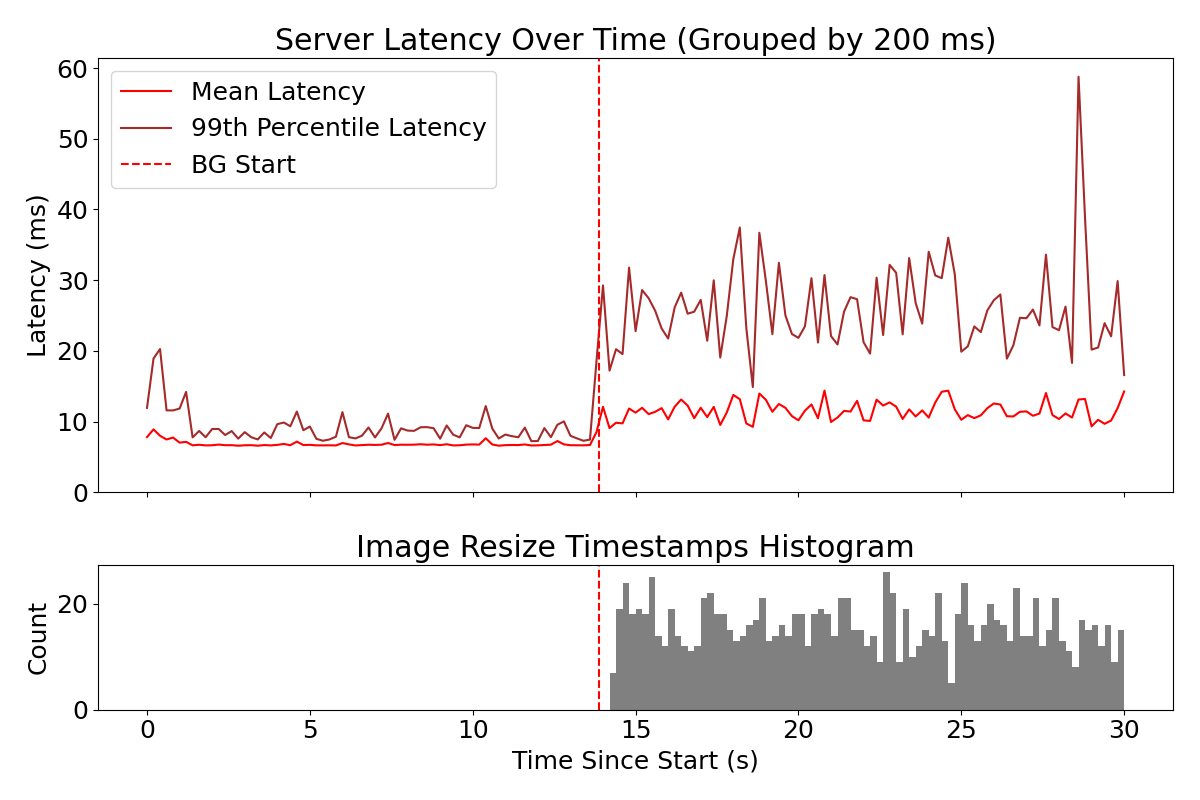
\includegraphics[width=\columnwidth]{graphs/kubernetes-unedited.png}
    \caption{In Kubernetes, running a BE has latency impacts on an LC with
    reservations}\label{fig:kubernetes-unedited}
\end{figure}
% In Kubernetes, running a BE has latency impacts on an LC with
%     reservations

Surprisingly, current popular scheduling systems fail to honor reservations.
$\autoref{fig:kubernetes-unedited}$ shows the latency of an endpoint in a web
application in Kubernetes that gets a user's feed, and the throughput of a BE
image resize job, both running on the same cores. The mean response latency
jumps from $\sim$7ms to $\sim$15ms after starting the BE.




%-------------------------------------------------------------------------------
\section{Problem}\label{s:problem}
%-------------------------------------------------------------------------------


\begin{figure}[t]
    \centering
    \begin{subfigure}[b]{0.49\columnwidth}
        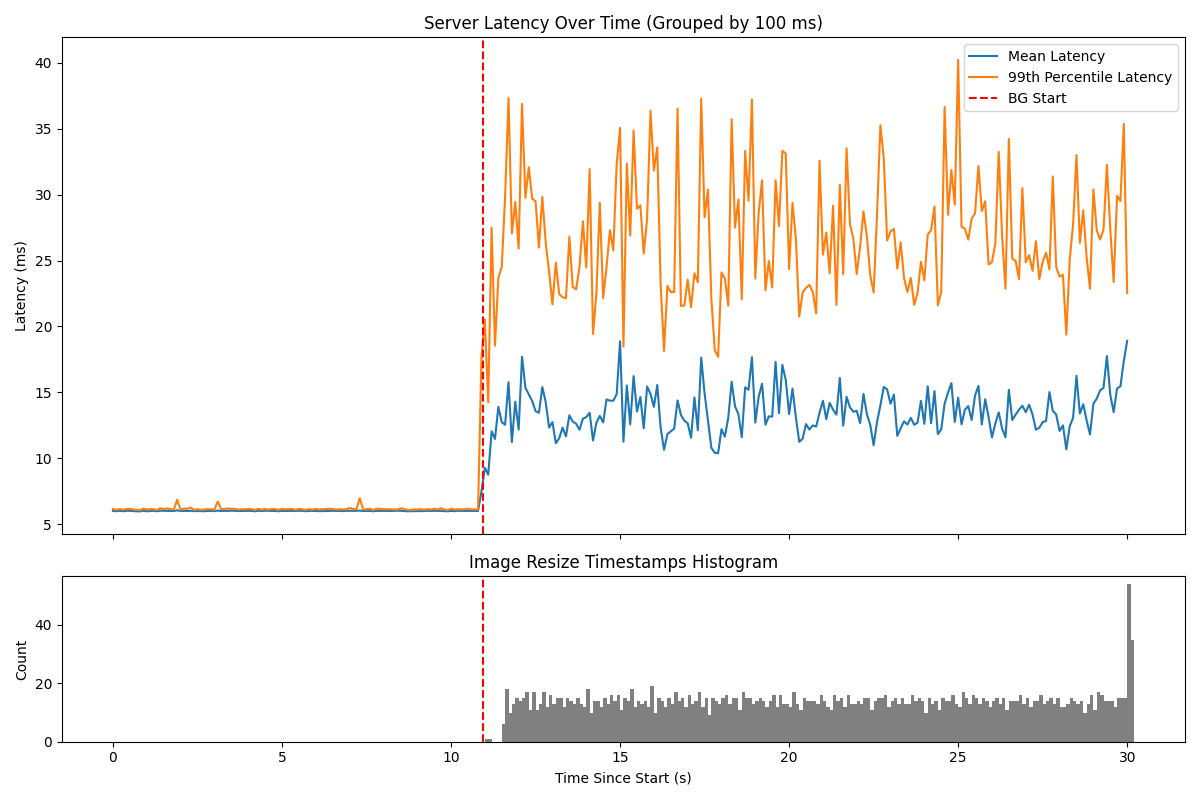
\includegraphics[width=\columnwidth]{graphs/srv-bg-unedited-low.png}
        \caption{Low load stetting, utilization before starting the BE tasks is
        around 85\%}\label{fig:srv-bg-unedited-low}
    \end{subfigure}
    \hspace{\fill}
    \begin{subfigure}[b]{0.49\columnwidth}
        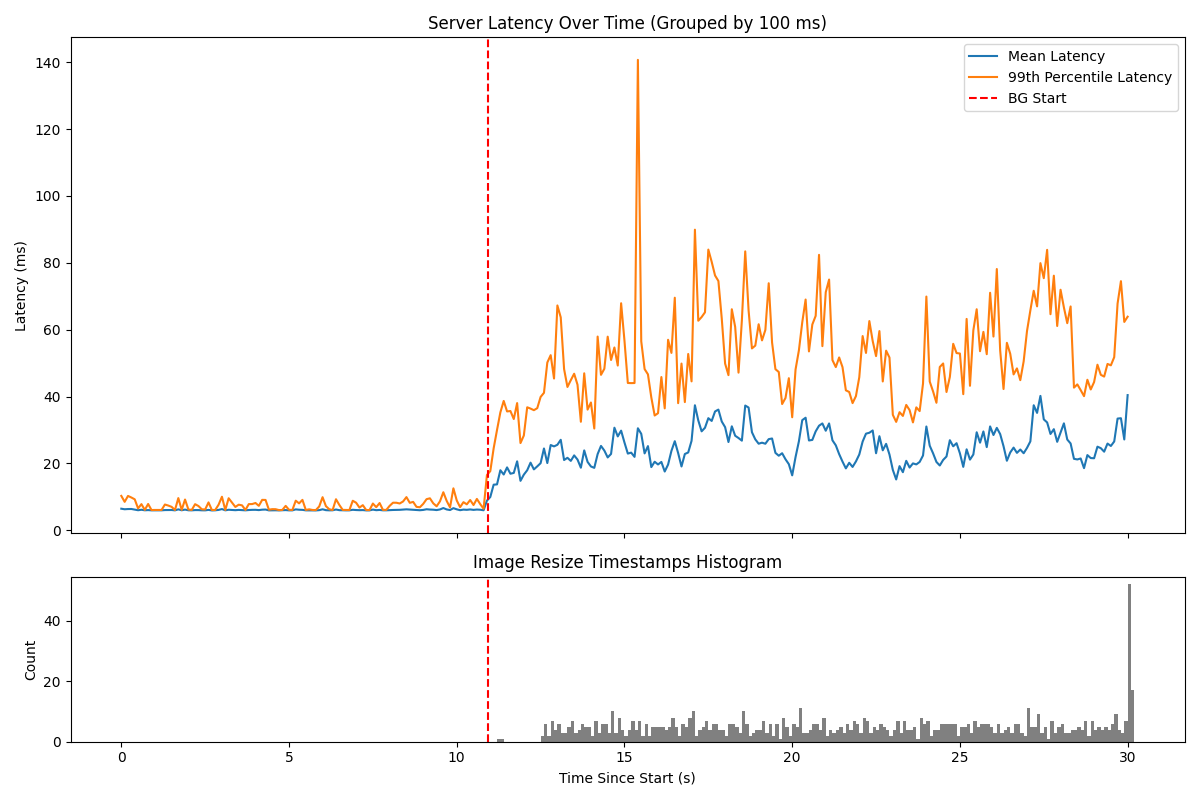
\includegraphics[width=\columnwidth]{graphs/srv-bg-unedited-high.png}
        \caption{High load setting, utilization before starting the BE tasks is
        around 95\%}\label{fig:srv-bg-unedited-high}
    \end{subfigure}
    \vspace{4pt}
    \caption{Latencies of the server and iteration counts of the background
    tasks in different load scenarios. Note the different y axis limits. The
    upper graphs show end-to-end request latencies, and the bottom graph is a
    histogram of completed iterations of the BE tasks}\label{fig:srv-bg-unedited}
\end{figure}

In order to understand more concretely where the isolation between the LC web
application and the BE image resize is failing in
\autoref{fig:kubernetes-unedited}, we reproduce the jump in latency we saw in
the application running on Kubernetes in a simpler benchmark. We run a simple
cpu-bound server with a pool of worker threads that we hit with an open-loop
remote client, and then start two BE workloads doing image resizing. We put the
LC server and the BE resize job each in their own \cgroups{} group, with weights
1 and 10000. \autoref{fig:srv-bg-unedited} shows the increase in latencies of
the LC server at two different baseline utilization levels. We see that even in
the lower baseline utilization case, where the server alone uses 85\%, mean
latencies spike up from steady at around 6ms to as high as 20ms, and much higher
for 99th percentile latencies.

\begin{figure}[t]
    \centering
    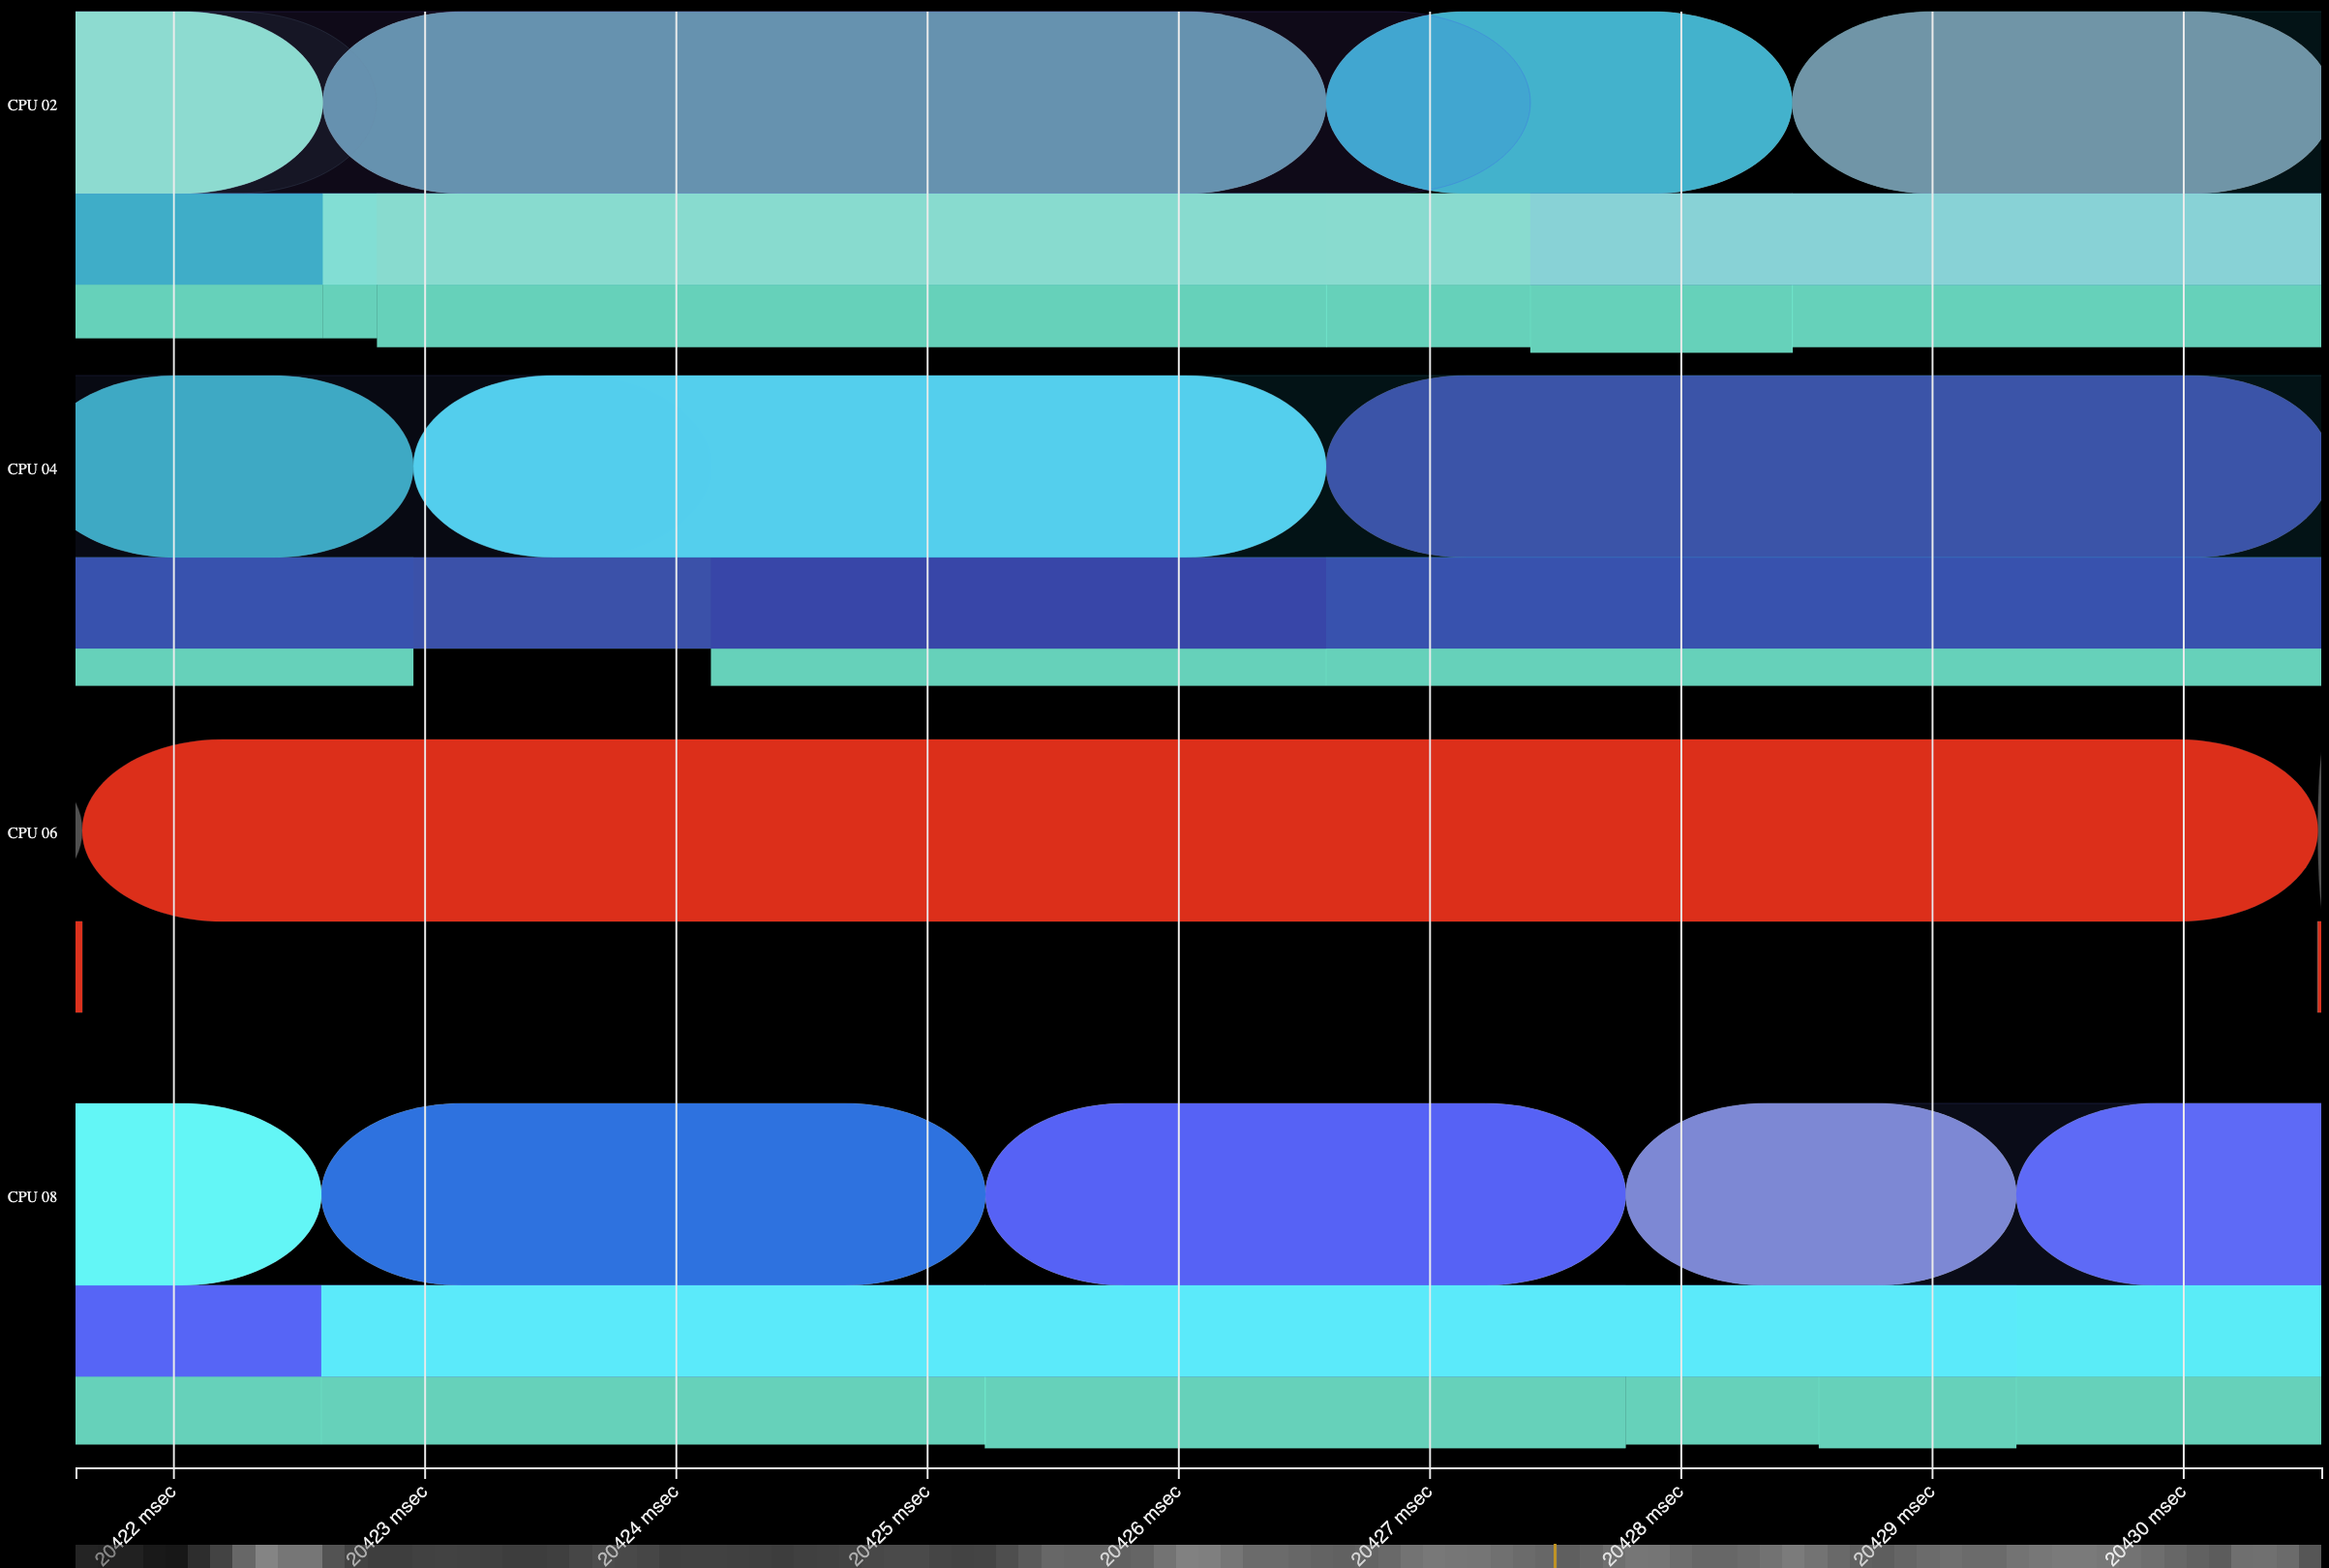
\includegraphics[width=\columnwidth]{graphs/schedviz-problem.png}
    \caption{Each thread is a different color. Circles represent which
    thread is running on that core, while rectangles underneath show waiting but
    runnable threads
    }\label{fig:schedviz-problem}
\end{figure}

Using this simplified experiment, we analyze perf traces of the scheduling
decisions, and visualize the trace using schedviz~\cite{schedviz-tool}, in order
to understand where the latency impact comes from.
\autoref{fig:schedviz-problem} shows a 10ms outtake of the resulting image. The
process running on each core is shown as a an oval, and queued processes are
shown as rectangles below. The root of the undesirable behavior is: on core 6,
the red process that is running the whole time is a BE process, whereas LC
threads, shown in varying shades of blue, are queued on the other cores. The
takeaway here is that the failure mode we observe is that \textit{one core is
running a BE process, while an LC process is waiting on another}.

Based on this observation, we explore more deeply the root of the issue that is
causing the poor behavior we see.

\subsection{Weights are only enforced locally}\label{ss:problem:mechanistic}

The reason this happens is that Linux maintains a separate runqueue on each
core, in order to avoid the synchronization overheads of accessing global state
for every scheduling decision. Within each runqueue, Linux's scheduler works to
maintain the correct ratio of received CPU time at each scheduling; but Linux
does not enforce the weight ratios across cores. This leads to the above failure
mode, where one core has no runnable high weight processes and thus runs a low
weight one, whereas another core has queued high weight processes. This problem
goes away when there are no BE processes, because cores try to steal work before
going idle.

\subsection{Enforcing weights across cores is
expensive}\label{ss:problem:cross-core-hard}

The root of the problem goes deeper than just a poor implementation: a
weight-based interface is at odds with machine-wide policy enforcement. In order
to strictly and globally enforce a processes weight, the scheduler would need to
synchronize at every scheduling decision: calculating whether a given process is
owed time globally requires knowing the total weight across all cores as well as
the sum of time that all the processes in the group have gotten. In increasingly
multi-core and multi-NUMA machines, synchronization is expensive; other work has
found that kernel lock contention is a bottleneck to performance at
scale.~\cite{afaas} This means that the overheads of maintaining global
invariants can quickly become prohibitive.


\subsection{Weights interact poorly with tick-based
scheduling}\label{ss:problem:quantum}

Even on a single runqueue, using very large weight differentials as an interface
to isolate LC and BE doesn't work well because preemption is tick-based. In a
weight based scheme, BE processes also get a fair share of the CPU. The problem
is that, when this happens, the BE process will interrupt any running LC process
for a whole tick. In Linux, hardware ticks are 4ms long. This means that an LC
thread processing a request may be interrupted for up to 4ms, provided the BE
process runs for that long before blocking. 4ms can be a large amount of time
for microservice workloads, whose SLOs are often in the low double digit or even
single digit ms realm.~\cite{sigmaos}




\section{Related work}

Some existing work focuses on isolating real-time applications in
Linux~\cite{rt-in-linux, state-rt-linux}, while Wasted Cores~\cite{wasted-cores}
focuses on the idle behavior of the Linux scheduler.

Other systems work around the kernel scheduler, by running primarily in
userspace~\cite{perfiso,caladan,skyloft}.

Linux's own \schedidle{} policy attempts to address this issue, but does not
fully solve it (running the microbenchmark using \schedidle{} still leads to an
increase in the mean latency from 6ms to 8).
\section{Approach \& Uniqueness}

In order to enforce reservations while running BE jobs opportunistically, our
approach uses priority scheduling instead of weights.

Enforcing priorities requires fewer global runqueue searches than weights do,
because they only need to happen on \textit{class boundary crossings}: on
\exit{}, when a core switches to running lower class processes after having
previously been running high class, and on \entry{}, when a core enqueues a high
class process. These checks ensure that a core $c$ running a BE thread $t$ knows
that there are no queued LC threads anywhere: the \exit{} check ensures theres
none when starting to run $t$, and the \entry{} check ensures if one wake up
while running $t$ it will interrupt $t$.

\begin{figure}[t]
    \centering
    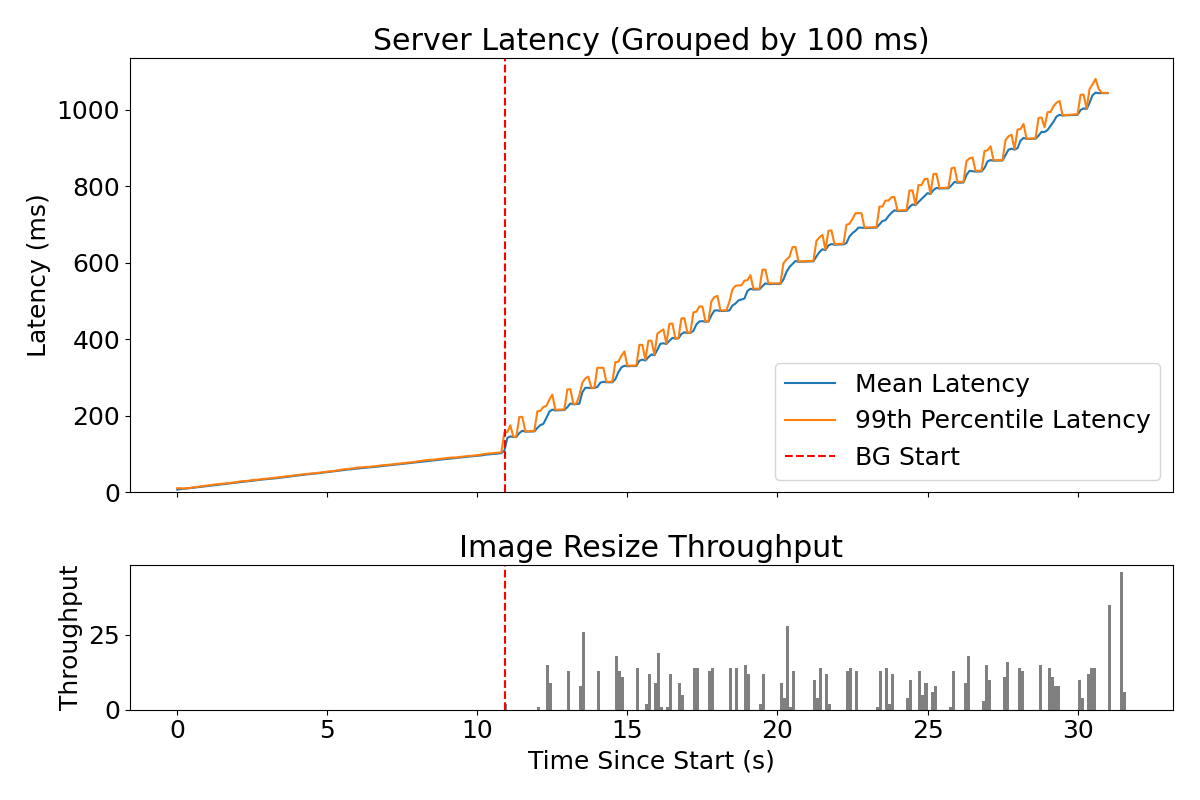
\includegraphics[width=\columnwidth]{graphs/overload-rt.png}
    \caption{when running the server in real time, throttling degrades
    its performance at high load}\label{fig:overload-rt}
\end{figure}


Linux already provides priority scheduling across scheduling classes, but it is
designed for real time applications: if these experience high load, Linux
throttles them in order to not starve the default class. We can see this
happening in \autoref{fig:overload-rt}, where throttling leads to spikes in the
BE task's throughput, and corresponding spikes in the server's latency.

We design a new scheduling class \beclass{} that sits at a lower priority than
\normalclass{}, which enforces LC applications' uncontended access to CPUs they
reserved. To enforce reservations under high load, without throttling the LCs or
killing the BEs, \beclass{} \textit{parks} BE processes, meaning the user-space
code never runs, only kernel-level services.
\section{Results}

\begin{figure}[t]
    \centering
    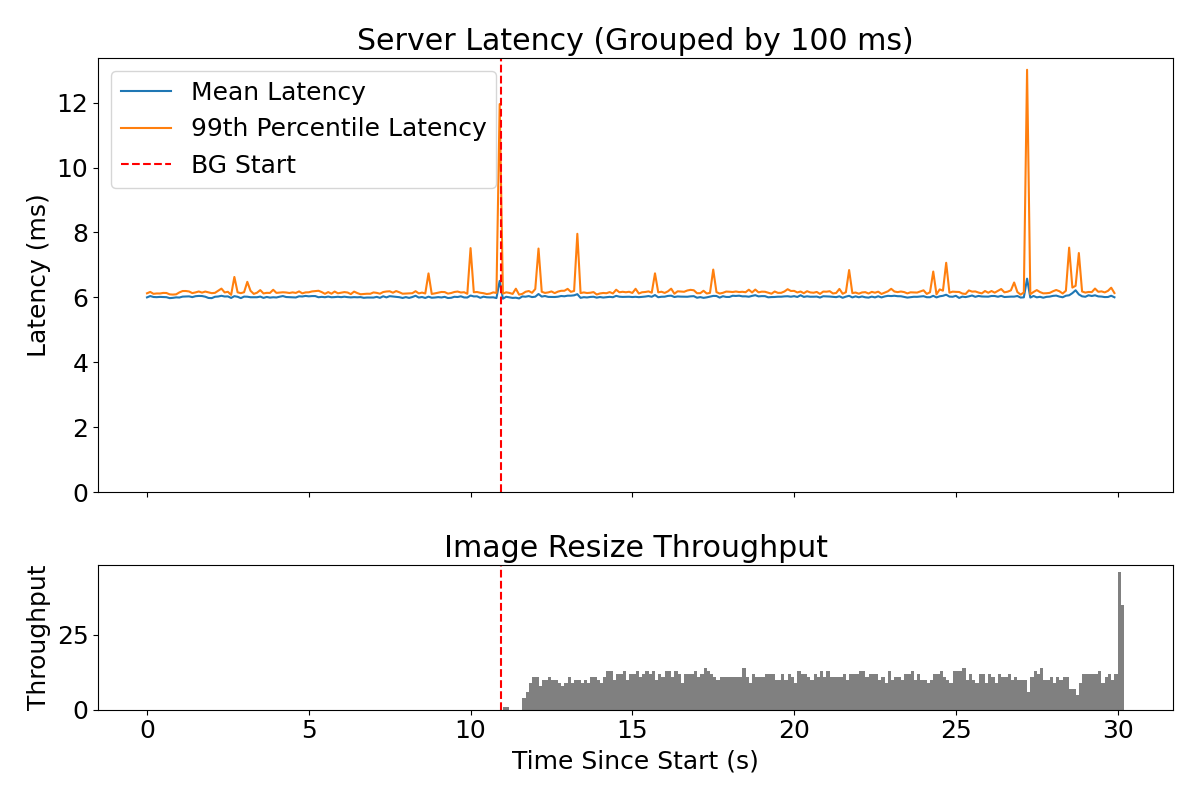
\includegraphics[width=\columnwidth]{graphs/srv-bg-schedbe-low.png}
    \caption{ \beclass{} does a good job of isolating the server's latencies
     from the load from best effort jobs}\label{fig:srv-bg-schedbe}
\end{figure}

We run the microbenchmark experiment from \autoref{fig:srv-bg-weight-cmp} using
\beclass{}. We can see the resulting performance in
\autoref{fig:srv-bg-schedbe}. As desired, the latency of the server remains
stable after the background tasks start, and the background task still runs (but
only in gaps where the core would otherwise be idle)

\begin{figure}[t]
    \centering
    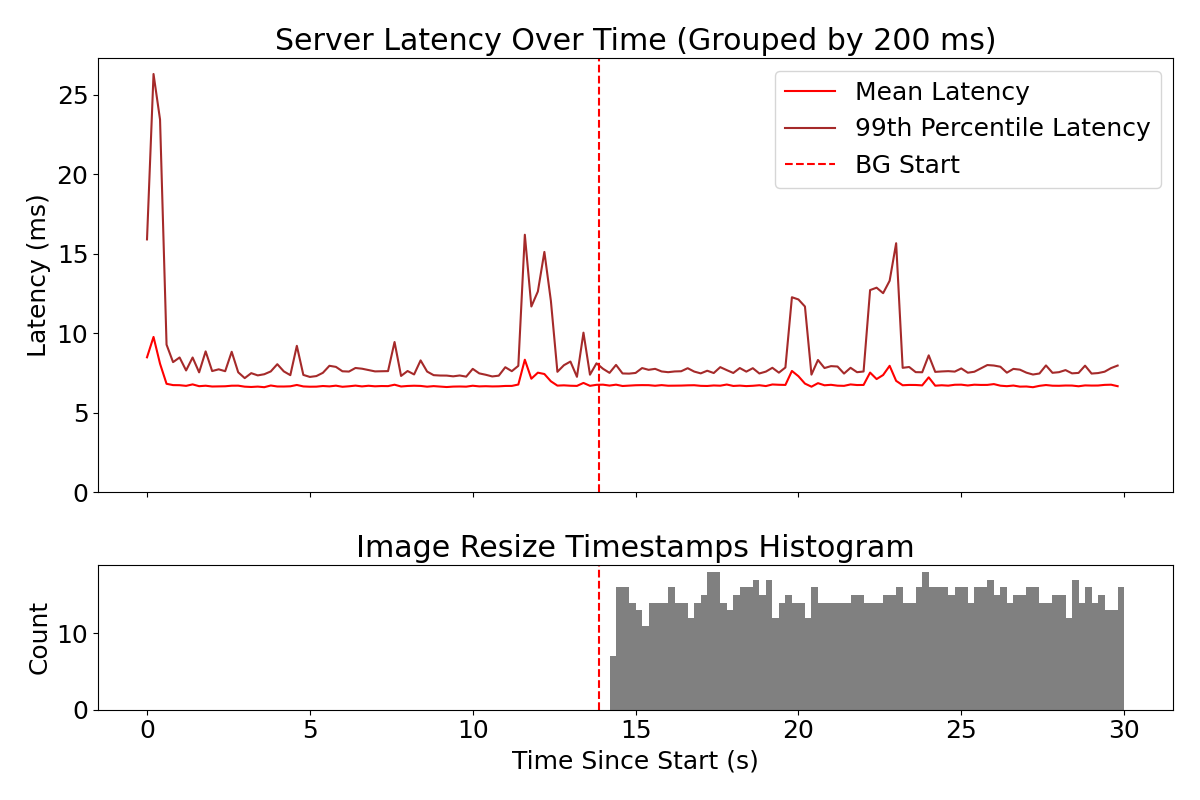
\includegraphics[width=\columnwidth]{graphs/kubernetes-schedbe.png}
    \caption{The same experiment as in \autoref{fig:kubernetes-unedited}, but
    running the BE as a \beclass{} task}\label{fig:kubernetes-schedbe}
\end{figure}

We also run the Kubernetes application from \autoref{fig:kubernetes-unedited}
using \beclass{}. The results are in \autoref{fig:kubernetes-schedbe}. We can
see that the baseline mean latency of the LC server stays around 7.4ms after
starting the the BE image resizing.

\begin{figure}[t]
    \centering
    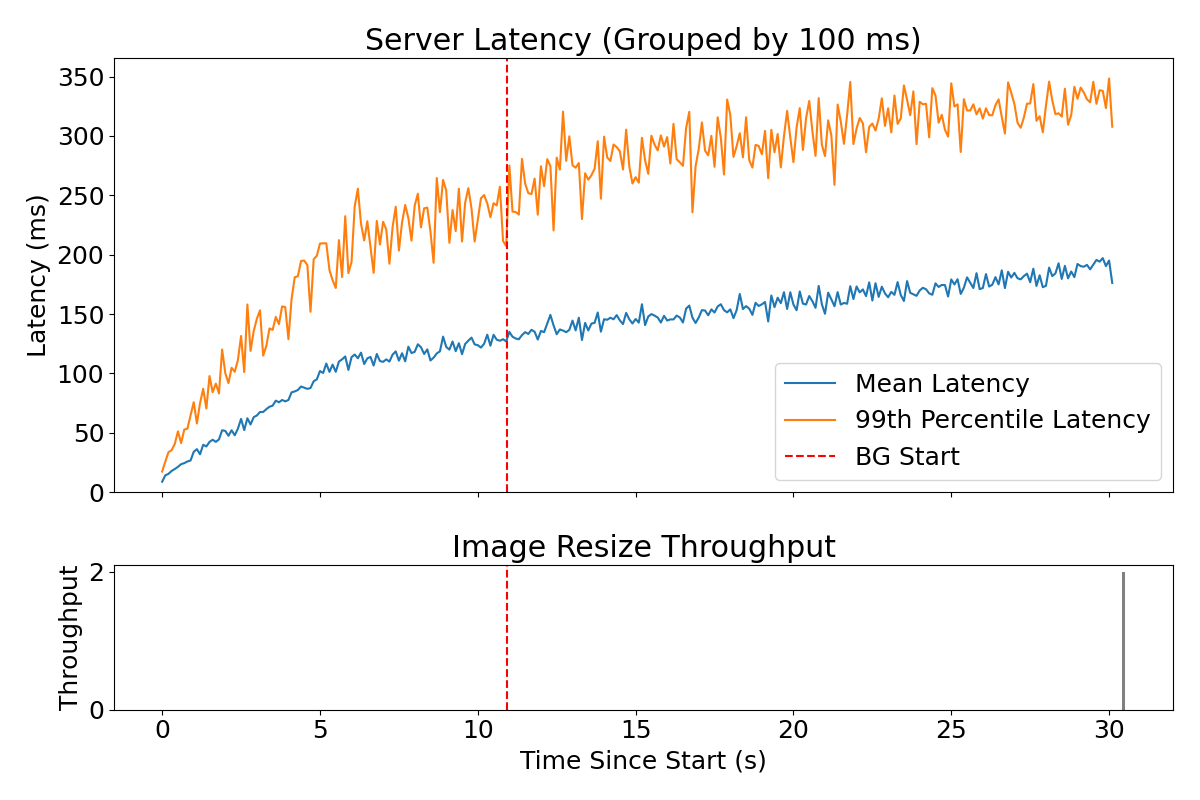
\includegraphics[width=\columnwidth]{graphs/overload-schedbe.png}
    \caption{BE in \schedbe{}, no throttling}\label{fig:overload-schedbe}
\end{figure}

\autoref{fig:overload-schedbe} shows how parking enables the latency critical
server to keep its reservation even under sustained extremely high load. We run
the same client load as \autoref{fig:overload-rt}, but now instead instead of
throttling the server, \schedbe{} parks the best effort processes. Notice that
the \schedbe{} image resize job does not make progress until the very end, when
the server is done processing the requests.

%-------------------------------------------------------------------------------
\section{Contributions}
%-------------------------------------------------------------------------------

This work identifies a serious limitation of \cgroups{} weights, they are unable
to effectively honor the reservations of LC applications in the presence BE
workloads, and shows that this is because Linux uses per-core runqueues. 

Instead, we propose an API that separates BE from LC by introducing \beclass{},
which requires fewer cross-core interactions than a weight-based approach, and
ensures that no BE is ever running when an LC is queued.

We implement this strict priority in Linux, and show that \beclass{} allows
\cgroups{} itself, as well as higher level applications like Kubernetes, to
ensure LC processes' access to their reserved cores while running BE workloads
opportunistically.



%-------------------------------------------------------------------------------
% \bibliography{paper.bib}
\printbibliography

%%%%%%%%%%%%%%%%%%%%%%%%%%%%%%%%%%%%%%%%%%%%%%%%%%%%%%%%%%%%%%%%%%%%%%%%%%%%%%%%
\end{document}
%%%%%%%%%%%%%%%%%%%%%%%%%%%%%%%%%%%%%%%%%%%%%%%%%%%%%%%%%%%%%%%%%%%%%%%%%%%%%%%%

%%  LocalWords:  endnotes includegraphics fread ptr nobj noindent
%%  LocalWords:  pdflatex acks
